%%%%%%%%%%%%%%%%%%%%%%%%%%%%%%%%%%%%%%%%%
% a0poster Landscape Poster
% LaTeX Template
% Version 1.0 (22/06/13)
%
% The a0poster class was created by:
% Gerlinde Kettl and Matthias Weiser (tex@kettl.de)
% 
% This template has been downloaded from:
% http://www.LaTeXTemplates.com
%
% License:
% CC BY-NC-SA 3.0 (http://creativecommons.org/licenses/by-nc-sa/3.0/)
%
%%%%%%%%%%%%%%%%%%%%%%%%%%%%%%%%%%%%%%%%%

%----------------------------------------------------------------------------------------
%	PACKAGES AND OTHER DOCUMENT CONFIGURATIONS
%----------------------------------------------------------------------------------------

\documentclass[a0,portrait]{a0poster}

\usepackage{multicol} % This is so we can have multiple columns of text side-by-side
\columnsep=100pt % This is the amount of white space between the columns in the poster
\columnseprule=3pt % This is the thickness of the black line between the columns in the poster

\usepackage[svgnames]{xcolor} % Specify colors by their 'svgnames', for a full list of all colors available see here: http://www.latextemplates.com/svgnames-colors
\usepackage{pgfpages}
\pgfpagesdeclarelayout{resize and center}
{
	\def\pgfpageoptionborder{0pt}
}
{
	\pgfpagesphysicalpageoptions
	{%
		logical pages=1,%
		physical height=\pgfpageoptionheight,%
		physical width=\pgfpageoptionwidth%
	}
	\pgfpageslogicalpageoptions{1}
	{%
		resized width=\pgfphysicalwidth,%
		resized height=\pgfphysicalheight,%
		border shrink=\pgfpageoptionborder,%
		center=\pgfpoint{.5215\pgfphysicalwidth}{.47\pgfphysicalheight}%
	}%
}
\pgfpagesuselayout{resize and center}[a2paper]

\usepackage{graphicx}
\usepackage{hyperref}
\usepackage{subcaption}
\usepackage{tikz}
\usepackage{float}
\usepackage{pgfplots}
\usepackage{hyperref}



\usepackage{times} % Use the times font
%\usepackage{palatino} % Uncomment to use the Palatino font

\usepackage{graphicx} % Required for including images
\graphicspath{{figures/}} % Location of the graphics files
\usepackage{booktabs} % Top and bottom rules for table
\usepackage[font=small,labelfont=bf]{caption} % Required for specifying captions to tables and figures
\usepackage{amsfonts, amsmath, amsthm, amssymb} % For math fonts, symbols and environments
\usepackage{wrapfig} % Allows wrapping text around tables and figures

\begin{document}

%----------------------------------------------------------------------------------------
%	POSTER HEADER 
%----------------------------------------------------------------------------------------

% The header is divided into three boxes:
% The first is 55% wide and houses the title, subtitle, names and university/organization
% The second is 25% wide and houses contact information
% The third is 19% wide and houses a logo for your university/organization or a photo of you
% The widths of these boxes can be easily edited to accommodate your content as you see fit

\begin{minipage}[b]{1.0\linewidth}
	\centering
\veryHuge \color{NavyBlue} \textbf{Unnecessarily Complicated Research Title} \color{Black}\\ % Title
%\Huge\textit{An Exploration of Complexity}\\[1cm] % Subtitle
\huge \textbf{John Smith \& James Smith}\\ % Author(s)
\huge University and Department Name\\ % University/organization
\end{minipage}
%
%\begin{minipage}[b]{0.10\linewidth}
%	\centering
%
\includegraphics[width=8cm]{images/others/iitm_logo.jpg} % Logo or a photo of you, adjust its dimensions here
%\end{minipage}

\vspace{1cm} % A bit of extra whitespace between the header and poster content

%----------------------------------------------------------------------------------------

\begin{multicols}{3} % This is how many columns your poster will be broken into, a poster with many figures may benefit from less columns whereas a text-heavy poster benefits from more

\section{Governing equations}
Continuity equation,
\begin{equation}
\frac{\partial \rho}{\partial t} + \nabla.(\rho \vec{v}) = 0
\label{eq:continuity}
\end{equation}
Navier-Stokes equation,
\begin{equation}
%{\partial{\vec{v}}\over{\partial t}} + ({\vec{v}} \cdot \nabla) {\vec{v}} = - {1\over\rho} \nabla p + \gamma\nabla^2{\vec{v}} + {1\over\rho}{\vec{F} }
\rho [\vec{v} + (\vec{v}.\nabla)\vec{v}] = \eta \nabla^2\vec{v}-\phi\nabla\mu - \nabla P
\label{eq:NS}
\end{equation}
Cahn-Hilliard convection-diffusion equation,
\begin{equation}
\frac{\partial \phi}{\partial t} = \nabla.(\phi \vec{v}) + \nabla.(M\nabla\phi)
\label{eq:CH}
\end{equation}
where $\phi$ is the phase field and M is \textit{mobility parameter} which plays the role of diffusivity.







\section{Lattice-Boltzmann method}
Instead of solving equations (\ref{eq:continuity})-(\ref{eq:CH}), the discrete Boltzmann equation is solved to simulate the flow of a Newtonian fluid.
\begin{equation}
f_{i}(\textbf{r}+\textbf{c}_{i}\Delta t, t+\Delta t) - f_{i}(\textbf{r},t) = -\frac{\Delta t}{\tau}(f_{i}-f_{i}^{eq})
\label{eq:f}
\end{equation}

\begin{equation}
g_{i}(\textbf{r}+\textbf{c}_{i}\Delta t, t+\Delta t) - g_{i}(\textbf{r},t) = -\frac{\Delta t}{\tau_{g}}(g_{i}-g_{i}^{eq})
\label{eq:g}
\end{equation}

Hydrodynamic variables are related to above velocity distribution functions by,
\begin{equation}
\rho \equiv \sum_{i} f_{i}, \quad \rho v_{\alpha} \equiv \sum_{i} c_{i\alpha} f_{i}, \quad \phi \equiv \sum_{i} g_{i}
\label{eq:fg}
\end{equation}

Also, 
\begin{equation}
\sum_{i} f_{i}^{eq} \equiv \rho, \quad \  \sum_{i} c_{i\alpha} f_{i}^{eq} \equiv rho v_{\alpha}, \sum_{i} g_{i}^{eq} \equiv \quad \phi 
\label{eq:fg}
\end{equation}
Expressions for equilibrium distribution functions are reported in \cite{paper:intertial_effects}.

\section{Spinodal decomposition}

Spinodal decomposition is a mechanism for the rapid unmixing of a mixture of liquids or solids from one thermodynamic phase, to form two coexisting phases. Refer Figure \ref*{fig:spinod} for the spinodal decomposition simulation where we started with each point having a random $\phi$ value where $ -1 \leq \phi \leq 1.  $
\begin{figure}[H]
	\centering
	\begin{subfigure}{4.2cm}            
		\frame{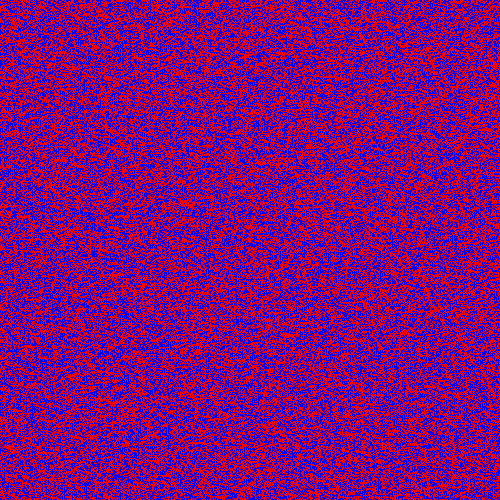
\includegraphics[width=4.2cm]{images/spinodal/0.png}}
		\caption{t = 0}
		\label{Fig:Data1}
	\end{subfigure}
	\begin{subfigure}{4.2cm}
		\centering
		\frame{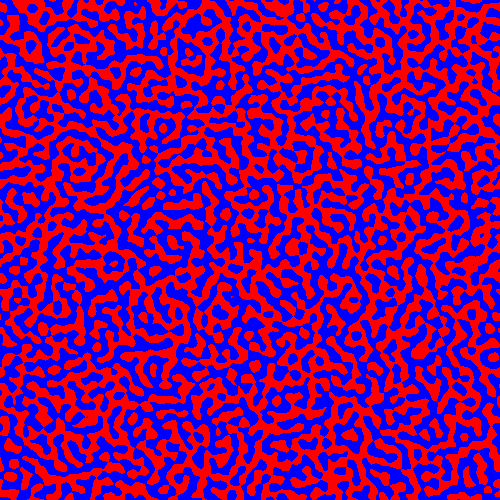
\includegraphics[width=4.2cm]{images/spinodal/1000.png}}
		\caption{t = 1000}
		\label{Fig:Data2}
	\end{subfigure}
	\begin{subfigure}{4.2cm}            
		\frame{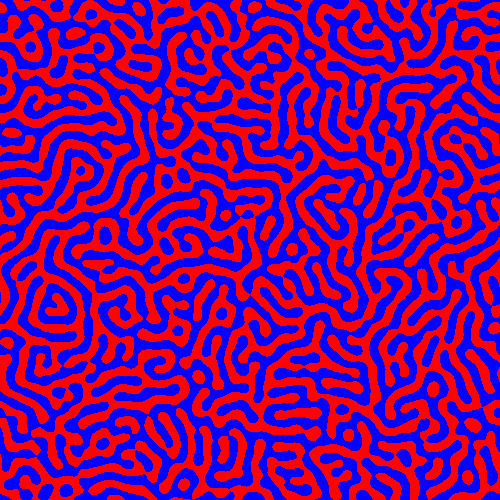
\includegraphics[width=4.2cm]{images/spinodal/10000.png}}
		\caption{t = 10000}
		\label{Fig:Data3}
	\end{subfigure}
	\begin{subfigure}{4.2cm}
		\centering
		\frame{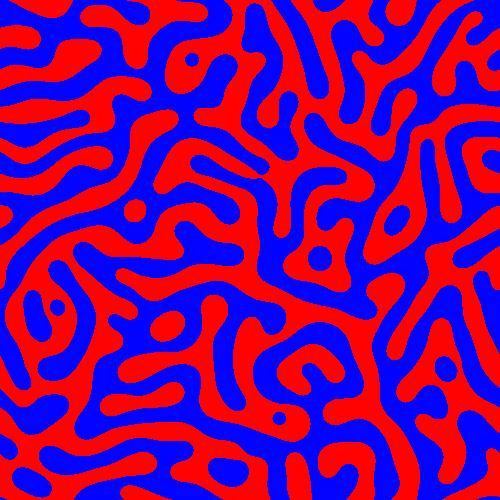
\includegraphics[width=4.2cm]{images/spinodal/100000.png}}
		\caption{t = 100000}
		\label{Fig:Data4}
	\end{subfigure}
	\caption{Spinodal decomposition simulation in a domain of 500 * 500 using Lattice Boltmann method. It can be seen that phases unmix to form sepearte clusters.}\label{fig:spinod}
\end{figure}
\begin{flushright}
	\href{https://www.youtube.com/watch?v=B9JiYVE437Y}{[Click here to see the video of the simulation.]}
\end{flushright}

\section{Surface tension}
Surface tension is the elastic tendency of a fluid surface which makes it acquire the least surface area possible. For any volume, sphere gives the least surface area. In the following simulation, a cubic volume of liquid is taken at t = 0. As expected, the droplets changes itself to a spherical droplet. (Refer Figure \ref{fig:surface_tension})

\begin{figure}[H]
	\centering
	\begin{subfigure}{4cm}            
		\frame{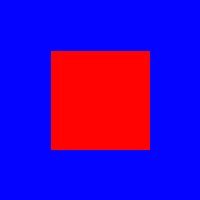
\includegraphics[width=4cm]{images/surface_tension/0.png}}
		\caption{At t = 0}
		\label{Fig:surface_initial}
	\end{subfigure}
	\begin{subfigure}{4cm}
		\centering
		\frame{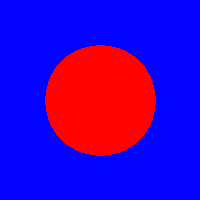
\includegraphics[width=4cm]{images/surface_tension/880000.png}}
		\caption{At equilibrium }
		\label{Fig:surface_final}
	\end{subfigure}
	\caption{Evolution of a square surface to a circular surface.}\label{fig:surface_tension}
\end{figure}

\section{Variation of phase phield close to interphase}
Close to interface, the phase field varies as a hyperbolic tangent with the normal cordinates to the interface, r. Simulation data was perfectly matching with the numberical solution given by \cite{arXiv:1104.0078}. (Refer Fig \ref*{fig:tanh}) \newline
\begin{equation}
\phi(r) = \phi_{eq}tan h(\frac{r}{\epsilon})
\end{equation}
where $\phi_{eq} = \sqrt{-a/b}$ and $\epsilon \equiv \sqrt{-2k/a}$ is the interface thickness
\begin{figure}[H]
	\begin{center}
		\begin{tikzpicture}
		\begin{axis}[
		width=7cm, % Scale the plot to \linewidth
		grid=major, % Display a grid
		grid style={dashed,gray!30}, % Set the style
		xlabel=$x$, % Set the labels
		ylabel=$\phi(x)/\phi_{eq}$,
		%x unit=\si{\volt}, % Set the respective units
		%y unit=\si{\ampere},
		legend style={at={( 1.01,1)}, anchor=north west}, % Put the legend below the plot
		x tick label style={rotate=90,anchor=east} % Display labels sideways
		]
		\addplot 
		% add a plot from table; you select the columns by using the actual name in
		% the .csv file (on top)
		table[x=X,y=Y,col sep=comma] {data/tanh.csv}; 
		\addlegendentry{Simulation data}
		\addplot [
		domain=0:150, 
		samples=100, 
		color=red,
		]
		%{abs(tanh(deg(x)))};
		{tanh((75-x)/2.2615822112761355)};
		\addlegendentry{Numerical Solution}
		\end{axis}
		
		\end{tikzpicture}
		\caption{Phase field profile along normal to interface of two already seperated phases }
		\label{fig:tanh}
	\end{center}
	
\end{figure}

\section{LB Method and Method of Lines}
Equation (\ref{eq:CH}) can be solved using method of lines, and the above simulations can be achieved. In this section, we compare various aspects of algorithms of LB method(LBM) and method of lines(MOL)
\subsection*{Time complexity}
Average time required for one iteration in both the algorithms was noted and plotted in Figure \ref*{fig:lbm_vs_mol_time}. It was noted that time for one iteration of MOL is almost equal to LB method with D2Q9 lattice. Time varies linearly with number of points for both the algorithms. Hence both shows time complexity of $\mathcal{O}(n)$
\begin{figure}[H]
	%\begin{center}
	\begin{subfigure}{7cm}
		\begin{tikzpicture}
		\begin{axis}[
		width=7cm, % Scale the plot to \linewidth
		grid=major, % Display a grid
		grid style={dashed,gray!30}, % Set the style
		xlabel=Number of points, % Set the labels
		ylabel=Average time for one iteration,
		%x unit=\si{\volt}, % Set the respective units
		%y unit=\si{\ampere},
		%legend style={at={( 1.01,1)}, anchor=north west}, % Put the legend below the plot
		x tick label style={rotate=90,anchor=east} % Display labels sideways
		]
		\addplot 
		[only marks]
		table[x=points,y=lbm,col sep=comma] {data/lbm_vs_mol_time.csv}; 
		%\addlegendentry{LB Method}
		\addplot
		[color=red] 
		[only marks]
		table[x=points,y=mol,col sep=comma] {data/lbm_vs_mol_time.csv}; 
		%\addlegendentry{Method of Lines}
		
		\end{axis}
		
		\end{tikzpicture}
		\caption{Average time for one iteration vary linearly for both the methods}
		\label{fig:lbm_vs_mol_time}
	\end{subfigure}
	\begin{subfigure}{7cm}
		\begin{tikzpicture}
		\begin{axis}[
		width=7cm, % Scale the plot to \linewidth
		grid=major, % Display a grid
		grid style={dashed,gray!30}, % Set the style
		xlabel=Time, % Set the labels
		ylabel=RMS Error,
		%x unit=\si{\volt}, % Set the respective units
		%y unit=\si{\ampere},
		legend style={at={( 1.05,0.6)}, anchor=north west}, % Put the legend below the plot
		x tick label style={rotate=90,anchor=east} % Display labels sideways
		]
		\addplot 
		[color=black]
		table[x=time,y=lbm,col sep=comma] {data/time_convergence.csv}; 
		\addlegendentry{LB Method}
		\addplot
		[color=red] 
		table[x=time,y=mol,col sep=comma] {data/time_convergence.csv}; 
		\addlegendentry{Method of Lines}
		
		\end{axis}
		
		\end{tikzpicture}
		\caption{Both the algorithms show same time for convergence}
		\label{fig:lbm_vs_mol_convergence}
	\end{subfigure}
	\caption{Time complexity and convergence analysis for LB method and method of lines}
	\label{fig:lbm_vs_mol}
	%\end{center}
	
\end{figure}
\subsection*{Space complexity}
Both the algorithms have same space complexity  $\mathcal{O}(n)$
\subsection*{Time for convergence}
It was noted that both the methods gives almost same result and error at a particular time and takes almost same time to converge to a solution. 
\section{Solid wall}
Bounce-back rules \cite{paper:bounce_back} are imposed along the boundary for impenetrability and no-slip boundary conditions. Also,
\begin{equation}
\vec{n}.\nabla\mu = 0
\end{equation}
For an equilibrium contact angle on an ideal solid wall, geometrical formulation is used for implemeting wetting condition \cite{paper:contact_angle}.
\begin{equation}
\phi_{i,j,1} = \phi_{i,j,3} + tanh(\frac{\pi}{2}-\theta) \xi
\end{equation}
where 
\begin{equation}
\xi = \sqrt{(\phi_{i+1,j,2}-\phi_{i-1,j,2})^{2}+(\phi_{i,j+1,2}-\phi_{i,j-1,2})^{2}}
\end{equation}
Considering the shape of the droplet, contact angle is given by\cite{paper:geometrical_contact_anngle} 
\begin{equation}
tan(\theta) = \frac{b_{0}}{2(R-a_{0})}
\end{equation}
where $ a_{0} $ is the droplet height and $ b_{0} $ is the wet length between the droplet and the wall,
\begin{equation}
R = \frac{a_{0}}{2} + \frac{b_{0}^{2}}{8a_{0}}
\end{equation}
\begin{figure}[H]
	\centering
	\begin{subfigure}{3cm}
		\frame{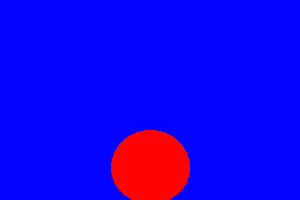
\includegraphics[height=2cm]{images/solid_wall/150.png}}
		\caption{Contact angle = xxx}
	\end{subfigure}
	\begin{subfigure}{2cm}            
		\frame{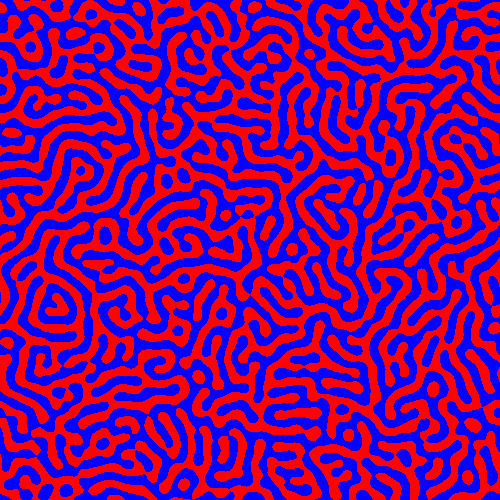
\includegraphics[width=2cm]{images/spinodal/10000.png}}
		\caption{Contact angle xxx}
		\label{Fig:Datsa3}
	\end{subfigure}
	
	\begin{subfigure}{2cm}
		\frame{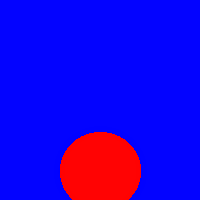
\includegraphics[width=2cm]{images/solid_wall/135.png}}
		\caption{Contact angle = xx$ ^{0} $}
	\end{subfigure}
	\begin{subfigure}{2cm}            
		\frame{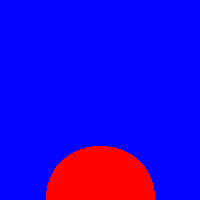
\includegraphics[width=2cm]{images/solid_wall/90.png}}
		\caption{Contact angle = 90$ ^{0} $}
		\label{Fig:Datsa1}
	\end{subfigure}
	\begin{subfigure}{2cm}            
		\frame{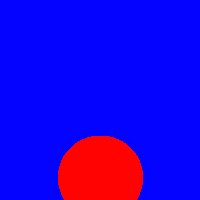
\includegraphics[width=2cm]{images/solid_wall/120.png}}
		\caption{Contact angle = $ 120^{0} $}
		\label{Fig:Datsase3}
	\end{subfigure}
	\begin{subfigure}{2cm}
		\frame{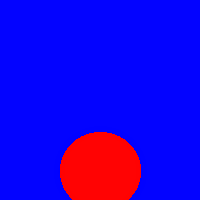
\includegraphics[width=2cm]{images/solid_wall/135.png}}
		\caption{Conatact angle = $ 135^{0} $}
	\end{subfigure}
	\begin{subfigure}{2.5cm}
		\frame{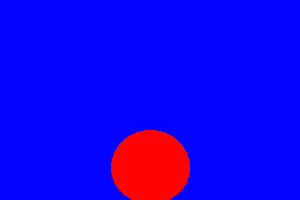
\includegraphics[height=2cm]{images/solid_wall/150.png}}
		\caption{Contact angle = 150$ ^{0} $}
	\end{subfigure}
	\caption{Droplets on solid wall with different contact angles }
	\label{fig:spinods}
\end{figure}

\section{Evaporation of a planar droplet}

To drive evaporation of the film we impose the boundary condition $\phi(z=z_{H},t)=\phi_{H}$, where $\phi_{H} < -\phi_{eq}$. This induces a gradient in the chemical potential field $\mu$. In response to this imabalance, the system reduces $\phi$, which curresponds to the evaporation of the film\cite{paper:evaporation}.
Phase field imbalance, $\Delta\phi_{H} \equiv -\phi_{eq} - \phi_{H}$
\newline
We performed simulations in a box consisting of  1 x 1 x 150 lattice sites. Periodic boundary conditions were set in the x and
y directions. A wall was located at $ z_{w} = 1 $, while the concentration
was fixed to a value $ \phi_{H}$ at $z_{H} = N_{z} $ to drive the system out of equilibrium. The initial height of the film was set to $z_{0} = 100$. 

\begin{figure}[H]
	\begin{center}
		\begin{subfigure}{6cm}
			\begin{tikzpicture}
			\begin{axis}[
			width=6cm, % Scale the plot to \linewidth
			grid=major, % Display a grid
			grid style={dashed,white!30}, % Set the style
			xlabel=$z$, % Set the labels
			ylabel=$\phi(x)/\phi_{eq}$,
			%x unit=\si{\volt}, % Set the respective units
			%y unit=\si{\ampere},
			%legend style={at={( 1.01,1)}, anchor=north west}, % Put the legend below the plot
			no markers,
			every axis plot/.append style={ultra thick},
			x tick label style={rotate=90,anchor=east} % Display labels sideways
			]
			\addplot 
			table[x=y,y=0.3,col sep=comma] {data/evaporation_different_phih.csv}; 
			\addlegendentry{0.3}
			\addplot 
			table[x=y,y=0.4,col sep=comma] {data/evaporation_different_phih.csv}; 
			\addlegendentry{0.4}
			\addplot 
			table[x=y,y=0.2,col sep=comma] {data/evaporation_different_phih.csv}; 
			\addlegendentry{0.2}
			\addplot 
			[color=cyan]
			table[x=y,y=0.1,col sep=comma] {data/evaporation_different_phih.csv}; 
			\addlegendentry{0.1}
			
			\end{axis}
			\end{tikzpicture}
			\caption{After 5 x $10^{6}$ simulation steps with different $\phi_{H}$}
			\label{fig:evaporation_tanh}
		\end{subfigure}
		\quad 
		\begin{subfigure}{6cm}
			\begin{tikzpicture}
			\begin{axis}[
			width=6cm, % Scale the plot to \linewidth
			grid=major, % Display a grid
			grid style={dashed,white!30}, % Set the style
			xlabel=$z$, % Set the labels
			ylabel=$\phi(x)/\phi_{eq}$,
			%x unit=\si{\volt}, % Set the respective units
			%y unit=\si{\ampere},
			legend style={at={( 1.01,1)}, anchor=north west}, % Put the legend below the plot
			no markers,
			every axis plot/.append style={ultra thick},
			x tick label style={rotate=90,anchor=east} % Display labels sideways
			]
			\addplot 
			table[x=y,y=1,col sep=comma] {data/evaporation_time.csv}; 
			\addlegendentry{$10^{5}$}
			\addplot 
			table[x=y,y=3,col sep=comma] {data/evaporation_time.csv}; 
			\addlegendentry{3 x $10^{5}$}
			\addplot 
			table[x=y,y=5,col sep=comma] {data/evaporation_time.csv}; 
			\addlegendentry{5 x $10^{5}$}
			\addplot 
			table[x=y,y=7,col sep=comma] {data/evaporation_time.csv}; 
			\addlegendentry{7 x $10^{5}$}
			
			\end{axis}
			\end{tikzpicture}
			\caption{Phase field profile at different time steps}
			\label{fig:evaporation_time}
			
		\end{subfigure}
		\caption{Phase field profile for the planar film evaporation. }
		\label{fig:evaporation_different_phih}
	\end{center}
	
\end{figure}


\section{Evaporation of a droplet on solid wall}
\bibliography{data/cite} 
\bibliographystyle{ieeetr}
\end{multicols}
\end{document}